\documentclass[titlepage = firstcover]{scrartcl}
\usepackage[aux]{rerunfilecheck}
\usepackage{fontspec}
\usepackage[main=ngerman, english, french]{babel}

% mehr Pakete hier
\usepackage{expl3}
\usepackage{xparse}
\usepackage{floatrow} 
\newfloatcommand{capbtabbox}{table}[][\FBwidth]%Table float box with bottom caption, box width adjusted to content

%Mathematik------------------------------------------------------
\usepackage{amsmath}   % unverzichtbare Mathe-Befehle
\usepackage{amssymb}   % viele Mathe-Symbole
\usepackage{mathtools} % Erweiterungen für amsmath
\usepackage[
  math-style=ISO,    % \
  bold-style=ISO,    % |
  sans-style=italic, % | ISO-Standard folgen
  nabla=upright,     % |
  partial=upright,   % /
]{unicode-math}% "Does exactly what it says on the tin."

% Laden von OTF-Mathefonts
% Ermöglich Unicode Eingabe von Zeichen: α statt \alpha

\setmathfont{Latin Modern Math}
%\setmathfont{Tex Gyre Pagella Math} % alternativ zu Latin Modern Math
\setmathfont{XITS Math}[range={scr, bfscr}]
\setmathfont{XITS Math}[range={cal, bfcal}, StylisticSet=1]

\AtBeginDocument{ % wird bei \begin{document}
  % werden sonst wieder von unicode-math überschrieben
  \RenewDocumentCommand \Re {} {\operatorname{Re}}
  \RenewDocumentCommand \Im {} {\operatorname{Im}}
}
\usepackage{mleftright}
\setlength{\delimitershortfall}{-1sp}

%Sprache----------------------------------------------------------
\usepackage{microtype}
\usepackage{xfrac}
\usepackage[autostyle]{csquotes}    % babel
\usepackage[unicode, pdfusetitle]{hyperref}
\usepackage{bookmark}
\usepackage[shortcuts]{extdash}
%Einstellungen hier, z.B. Fonts
\usepackage{booktabs} % Tabellen

%Defininierte funktionen
\DeclareMathOperator{\f}{xyz}

\ExplSyntaxOn % bequeme Syntax für Definition von Befehlen

\NewDocumentCommand \I {} {         %Befehl \I definieren,keine Argumente
  \symup{i}                         %Ergebnis von \I
} 
\NewDocumentCommand \dif {m} % m = mandatory (Pflichtargument für \dif)
{
  \mathinner{\symup{d} #1}
}

\ExplSyntaxOff % Syntax wieder ausschalten. Wichtig!

 
\subject{Versuchnummer: 803}
\title{Das Hooksche Gesetz}
\author{Marcel Kebekus \and Konstantin Mrozik}
\date{%
  Durchführung: 22.10.2019 \\
  Abgabe: 29.10.2019
  }
  
\makeatletter
\newcommand{\mathleft}{\@fleqntrue\@mathmargin0pt}
\newcommand{\mathcenter}{\@fleqnfalse}
\makeatother


\begin{document}
\maketitle
\thispagestyle{empty}
\tableofcontents
\clearpage
\setcounter{page}{1}

\newpage

\section{Theorie}
\label{sec:Theorie}
Das Hooksche Gesetz beschreibt die elastische Verformung, welche sich
proportinoal zur Kraft verhält.
Bei einem Federsystem führt man dabei die Federkonstante $D$ als Proportionalitätsfaktor ein.\\
Es gilt:
\\
\begin{equation}
  \vec{F_{\text{D}}}=-D \cdot \vec{x} \iff D=\frac{\lvert\vec{F_{\text{D}}}\rvert}{\lvert\increment\vec{x}\rvert}
  \label{eqn:Formel}
\end{equation}
\\
Das Hooksche Gesetz gilt nicht mehr, sobald die Feder überspannt wird, sie also den Bereich der
elastischen Verformung verlässt.


\section{Versuchanordnung}
\label{sec:Versuchsanordnung}
Eine Feder mit einer unbekannten Federkonstaten $D$ wird an einem festen Gestell aufgehängt
und mit einem Faden über eine Umlenkrolle an einem Maker am Zollstock befestigt. 
Die Kraft auf die Feder wird mit einem elektroschen KRaftmesser über die Aufhängung der Feder gemessen.


\section{Versuchsdurchführung}
\label{sec:Versuchsdurchführung}
Im Versuche wird der Marker am Zollstocke um verschiedene $\increment x$ verschoben, um die Feder
auszulenken.
Zu den abgelesenen $\increment x$ Werten wird die jeweilige zugehörige Kraft $F_{\text{D}}$ notiert.
Es werden 10 verschiedene Auslenkungen vermessen, dabei wird der Bereich der elastischen Verformung nicht verlassen.

\newpage

\section{Auswertung}
\label{sec:Auswertung}
Mithilfe des Hook'schen Gesetzes lässt sich aus der Auslenkung $\increment x$ und der jeweilige
Kraft $F_{\text{D}}$ die Federkonstante $D$ berechnen.\\
Es gibt 2 Möglichkeiten die Federkonstante $D$ zu ermitteln:

\begin{enumerate}
  \item Aus der Federkonstanten der verschieden Messdaten lässt sich der Mittelwert $\bar{D}$ bilden und die dazu passende 
  Standartabweichung $\sigma_{\bar{x}}$

\begin{table}[h]
  \centering
  \caption{Messdaten mit errechneter Federkonstante $D$}
  \label{tab:table}
  \begin{tabular}{c c c}
    \toprule
  $ \increment x \:/\:m$  & $F \:/\: N$ (mit Fehler 1\%)  & $D \:/\: \frac{N}{m}$  \\
    \midrule
  6  &	0.18 & 3.0  \pm 0.075  \\	
  12 &	0.36 & 3.0  \pm 0.075	\\
  18 &	0.53 & 2.944 \pm 0.073	\\
  24 &	0.71 & 2.958 \pm 0.073	\\
  30 &	0.89 & 2.966 \pm 0.074 \\
  36 &	1.07 & 2.972 \pm 0.074 \\
  42 & 	1.25 & 2.976 \pm 0.074 \\
  48 &	1.44 & 3.0 \pm 0.075 \\
  54 &	1.61 & 2.981 \pm 0.074\\
  58 &	1.73 & 2.982 \pm 0.074 \\
  \bottomrule
\end{tabular}
\end{table}



Für den Mittelwert $\bar{D}$ gilt dann:
\mathleft
\begin{equation*}
  \bar{D} = \frac{1}{10} \sum_{i=1}^{10} D_\text{i} = 2.978 \pm 0.024
\end{equation*}
\mathcenter
\newpage



  \item In der Theorie \eqref{eqn:Formel} ist erkannbar, dass eine lineare Abhängigkeit zwischen der Kraft und der Auslenkung besteht.
  Trägt man diese in einem Diagramm auf, so bildet die Steigung der Geraden die Federkonstante $D$.
\end{enumerate}

\begin{figure}[h]
  \centering
  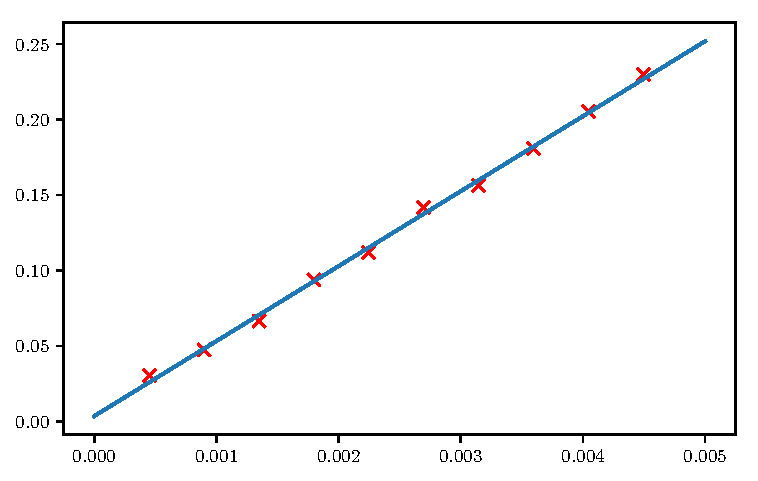
\includegraphics[width=\textwidth]{build/plot.pdf}
  \caption{Messdaten mit Ausgleichsgraden}
  \label{fig:Plot}
\end{figure}

































%%%%%%%%%%%%%%%%%%%%%%%%%%%%%%%%%%%%%%%%%%%%%%%%%
\begin{figure}
  \begin{floatrow}
  \ffigbox{
  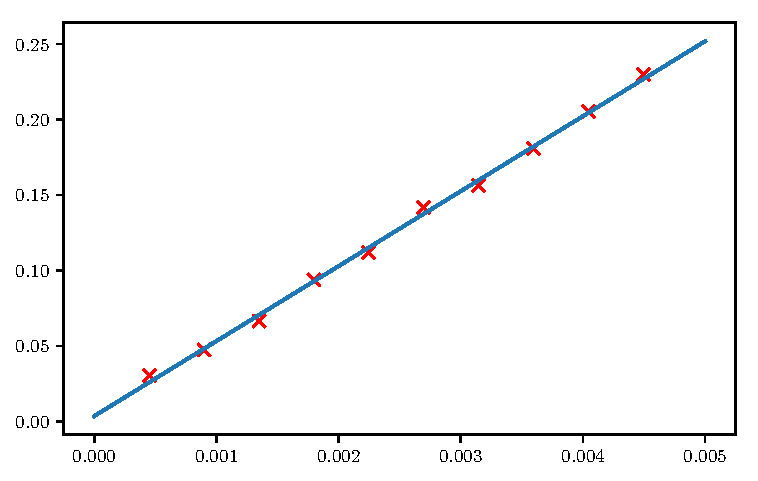
\includegraphics[width=\textwidth/2]{build/plot.pdf}
  \label{fig:Plot}
  }{ 
    \caption{Eine Beschreibung}
    }
  \capbtabbox{
    \begin{tabular}{c c c}
    \toprule
  $ \increment x \pm 0,001m $ & $F$ (mit Fehler 1\%)  & $D$  \\
    \midrule
  6  &	0.18 & 0 \\	
  12 &	0.36 & 0	\\
  18 &	0.53 & 0	\\
  24 &	0.71 & 0	\\
  30 &	0.89 & 0 \\
  36 &	1.07 & 0 \\
  42 & 	1.25 & 0 \\
  48 &	1.44 & 0 \\
  54 &	1.61 & 0 \\
  58 &	1.73 & 0 \\
  \bottomrule
\end{tabular}
  }{\caption{Tabelle}}
\end{floatrow}
\end{figure}

\end{document}


